%   Autor: Axel Uriel Padilla Amezcua
%
%	Este template fue originalmente diseñado para emplearse en el curso de Laboratorio de Mecánica, impartido por la Dra. Areli Huanosta Gutiérrez en la Facultad de Ciencias de la UNAM. El template incluye un archivo de bibliografía .bib que contiene la información de los libros de referencia del curso. Cualquier comentario o sugerencia sobre el template puede ser enviado al correo del autor:
%	
%	axelpadilla@ciencias.unam.mx

% --- Paquetes ---

% Básicos
\documentclass[letterpaper]{article}
\usepackage[english, spanish, mexico, es-noitemize]{babel}
\usepackage{pdflscape}

% Matemáticas avanzadas
\usepackage[tbtags]{amsmath}
\usepackage{amssymb, amsthm, mathtools, physics}
\usepackage[nolimits]{cmupint}% Integrales rectas
\usepackage{booktabs}
\usepackage{longtable}
\usepackage[table,xcdraw]{xcolor}
%\usepackage{siunitx}% Unidades del SI

% Selección de fuente: Descomente el segundo bloque y comente el primero para cambiar entre las dos fuentes

% Latin Modern, fuente estándar
\usepackage{lmodern}
\usepackage[T1]{fontenc}

% TeX Gyre Schola con fouriernc para mates consistentes con la fuente
%\usepackage{fouriernc}
%\usepackage[scale=0.92]{tgschola}
%\usepackage[T1]{fontenc}

% Configuración del documento
\usepackage[margin=1in, top=1.25in, headheight=2\baselineskip, headsep=\baselineskip]{geometry}
\usepackage{fancyhdr}
\usepackage[pdfusetitle, colorlinks]{hyperref}
\usepackage[shortlabels, inline]{enumitem}
\usepackage{multicol, array}
\usepackage{titlesec}
\usepackage[titles]{tocloft}
\usepackage{xcolor, xpatch, calc}

% Gráficos
\usepackage{graphicx, booktabs, wrapfig, pdfpages}
\usepackage{pgfplots}
\usepackage[framemethod=tikz]{mdframed}
\usepackage[outline]{contour}
\usepackage[hang, labelfont=bf, labelsep=period, margin=0.5in]{caption}
\usepackage{subcaption}
\usepackage{tikz}
\usetikzlibrary{mindmap}
\documentclass[tikz,border=10pt,multi]{standalone}
\usepackage{forest}
\usetikzlibrary{shadows}
\usepackage{tikz-uml}

% Bibliografía
\usepackage[backend=biber]{biblatex}
\usepackage{csquotes}
\addbibresource{repbib.bib}

% Texto de prueba
\usepackage{lipsum}


\usepackage{listings}
\usepackage{color}

\definecolor{dkgreen}{rgb}{0,0.6,0}
\definecolor{gray}{rgb}{0.5,0.5,0.5}
\definecolor{mauve}{rgb}{0.58,0,0.82}

\lstset{frame=tb,
  language=Java,
  aboveskip=3mm,
  belowskip=3mm,
  showstringspaces=false,
  columns=flexible,
  basicstyle={\small\ttfamily},
  numbers=none,
  numberstyle=\tiny\color{gray},
  keywordstyle=\color{blue},
  commentstyle=\color{dkgreen},
  stringstyle=\color{mauve},
  breaklines=true,
  breakatwhitespace=true,
  tabsize=3
}

% --- Información del documento ---

\title{\mytitle}
\author{\myauthor}
\date{\thedate}

\newcommand{\mytitle}%
	{Práctica 1}
	
\newcommand{\mysubtitle}%
	{Medidas repetibles y su incertidumbre}

\newcommand{\myauthor}%
	{Axel Uriel Padilla Amezcua}

\newcommand{\myemail}%
	{\href{mailto:axelpadilla@ciencias.unam.mx}%
	{\texttt{axelpadilla@ciencias.unam.mx}}}%

\newcommand{\thedate}%
	{\today}

\newcommand{\thesubject}%
	{ANÁLISIS Y DISEÑO DE SISTEMAS}

\newcommand{\firstinstitute}%
	{Escuela Superior de Computo}

\newcommand{\secondinstitute}%
	{Instituto Politécnico Nacional}

\newcommand{\shortinstitute}%
	{Escuela Superior de Computo}

% --- Configuraciones adicionales ---

% Idioma en el preámbulo
\selectspanish

% Librerías de pgfplots
\usepgfplotslibrary{colormaps}

% Librerías de tikz
\usetikzlibrary{babel, calc, scopes, intersections, angles, quotes, arrows, arrows.meta, backgrounds, shapes.geometric, patterns, shadows, perspective, external}

% Descomentar la siguiente línea para externalizar gráficos
%\tikzexternalize

% Versión de PGFplots
\pgfplotsset{compat=newest}

% Definición de estilos de Tikz, etc.
\tikzset{%
	% Configuraciones de tikz particulares del documento, como estilos de nodos y dibujos
	font = {\selectfont},
	frame/.style={thin, dashed, lightgray, line cap=round, rounded corners=5pt}
}

% Grosor de contorno adicional (para emplearse en gráficos)
\contourlength{1pt}

% Directorios de gráficos
\graphicspath{{imágenes/}{escudos/}}

% Todos los enlaces del documento en negro
\hypersetup{allcolors=black}

% Listas personalizadas
\setlist[enumerate, 1]{%
	label=\textbf{\color{\emphcolor}\arabic*.},
	labelindent=\parindent,
	itemindent=*,
	ref=\textbf{\arabic*}
}
\setlist[enumerate, 2]{%
	label=\textbf{\color{\emphcolor}(\alph*)},
	itemindent=*,
	ref=\textbf{(\alph*)}
}
\setlist[enumerate, 3]{%
	label=\color{\emphcolor}\roman*.,
	itemindent=*,
	ref=\roman*
}

% Redefinición de "y otros" en la bibliografía
\DefineBibliographyStrings{spanish}{andothers={et~al\adddot}}

% Personalización de ToC
\renewcommand{\cftdotsep}{1}
\renewcommand{\cftsecleader}{\cftdotfill{\cftdotsep}}
\renewcommand{\cftsecpresnum}{\color{\emphcolor}}
\renewcommand{\cftsecaftersnum}{.}
\setlength{\cftsecindent}{25pt}
\renewcommand{\cftsecafterpnum}{\hspace*{25pt}}
\setlength{\cftbeforesecskip}{\baselineskip/2}

% --- Comandos de mate adicionales ---

\newcommand{\rtwovec}[2]{% Vectores columna en R^2 
	\begin{bmatrix*}[r]
		#1 \\ #2 
	\end{bmatrix*}
}

\newcommand{\rthreevec}[3]{% Vectores columna en R^3
	\begin{bmatrix*}[r]
		#1 \\ #2 \\ #3
	\end{bmatrix*}
}

\newcommand{\uvec}[1]{% Vectores unitarios (con gorrito)
	\textbf{\^{#1}}
}

\newenvironment{amatrix}[2]{% Matices aumentadas
	\left[\begin{array}{@{}*{#1}{r}|*{#2}{r}@{}}
	}%
	{
	\end{array}\right]
}

\DeclareMathOperator{\mcd}{mcd}% Máximo común divisor
\DeclareMathOperator{\midd}{med}% Número medio

% Descomentar esta línea si se elige fouriernc para la fuente matemática y emplear en vez de \nabla
%\newcommand{\Nabla}{\scalebox{1.075}{$\nabla$}}

% --- Diseño de documento ---

% Colores
% \definecolor{emphcolor}{HTML}{0B4166}% Color de énfasis personalizado
\newcommand{\emphcolor}{gray}% Escribir emphcolor dentro de las llaves, si se define

% Longitudes
%\setlength{\columnsep}{0.5in}% Separación entre columnas

% Diseño de títulos de sección
\titleformat{\section}[hang]
{\thetitle.}{\widthof{\ }}{\Large\color{\emphcolor}}

% Título de documento
\newcommand{\cover}{%
	\thispagestyle{plain}
	\begin{center}
		\Large\textbf{\textcolor{\emphcolor}{\mytitle}} \\
		\LARGE\textbf{\mysubtitle}
		\bigskip
		
		\normalsize\myauthor \\
		\small\myemail
		\medskip
		
		\normalsize\firstinstitute \\ 
		\secondinstitute
		\medskip
		
		\normalsize\thedate \\
	\end{center}%
}

% Comandos para ingresar keywords en el abstract
\newcommand{\espkeywords}{\noindent\textit{Palabras clave:\ }}
\newcommand{\engkeywords}{\noindent\textit{Keywords:\ }}

% Tipos de columna útiles
\newcolumntype{P}[1]{>{\centering\arraybackslash}p{#1}}
\newcolumntype{M}[1]{>{\centering\arraybackslash}m{#1}}
\newcolumntype{R}[1]{>{\arraybackslash}m{#1}}

% Rediseño del estilo plain
\fancypagestyle{plain}{%
	\renewcommand{\headrulewidth}{0pt}
	
	\fancyhf{}
	\fancyfoot[c]{%
		\begin{tabular}{M{1em}@{}M{2em}@{}M{1em}}
			\textcolor{\emphcolor}{$\boldsymbol{-}$}
			& \thepage &
			\textcolor{\emphcolor}{$\boldsymbol{-}$}
		\end{tabular}
	}
}

% Diseño de los encabezados y pies de página
\pagestyle{fancy}

\renewcommand{\headrulewidth}{1pt}% Ancho de la regla en el encabezado
\xpretocmd\headrule{\color{\emphcolor}}{}{\PatchFailed}% Cambio de color de la regla en el encabezado

\fancyhf{}
\fancyhead[l]{%
	\begin{tabular}{@{}R{2.25em}@{}R{\widthof{\shortinstitute\ }}}
		
\includegraphics[height=.25in]{fcunam}% Escudo de la instittución
		& \shortinstitute
	\end{tabular}
}
\fancyhead[r]{%
	\textit{\thesubject}% Nombre de la asignatura
}
\fancyfoot[c]{%
	\begin{tabular}{M{1em}@{}M{2em}@{}M{1em}}
		\textcolor{\emphcolor}{$\boldsymbol{-}$}
		& \thepage &
		\textcolor{\emphcolor}{$\boldsymbol{-}$}
	\end{tabular}
}

\definecolor{backcolour}{rgb}{0.95,0.95,0.92}
    \definecolor{codegreen}{rgb}{0,0.6,0}
    
    % Define a custom style
    \lstdefinestyle{myStyle}{
        backgroundcolor=\color{backcolour},   
        commentstyle=\color{codegreen},
        basicstyle=\ttfamily\footnotesize,
        breakatwhitespace=false,         
        breaklines=true,                 
        keepspaces=true,                 
        numbers=left,       
        numbersep=5pt,                  
        showspaces=false,                
        showstringspaces=false,
        showtabs=false,                  
        tabsize=2,
    }

    \lstset{style=myStyle}

% --- Inicio del documento ---

\begin{document}

    \begin{titlepage}
  \thispagestyle{empty}
  \begin{minipage}[c][0.17\textheight][c]{0.25\textwidth}
    \begin{center}
    \hspace*{-13mm}
      
\includegraphics[ height=5cm]{escudos/unam.png}
    \end{center}
  \end{minipage}
  \begin{minipage}[c][0.195\textheight][t]{0.75\textwidth}
    \begin{center}
      \vspace{0.3cm}
             {\color{black}\textsc{\large Instituto Politécnico Nacional} }\\[0.5cm]
             \vspace{0.3cm}
                    {\color{black}\hrule height3pt}
                    \vspace{.2cm}
                           {\color{black}\hrule height2pt}
                           \vspace{.8cm}
                           \textsc{Escuela Superior de Computo}\\[0cm] %
    \end{center}
  \end{minipage}
  \begin{minipage}[c][0.81\textheight][t]{0.25\textwidth}
    \vspace*{5mm}
    \begin{center}
      \hskip0.5mm
             %{\color{purple}\vrule width1pt height13cm }
             \vspace{5mm}
             \hskip2pt
                 {\color{black}\vrule width3pt height13cm}
                 \hskip2mm
                     {\color{black}\vrule width1pt height13cm} \\
                     \vspace{5mm}
                     \hspace*{2mm}
                     
\includegraphics[height=4cm]{escudos/fcunam.png}
    \end{center}
  \end{minipage}
  \begin{minipage}[c][0.81\textheight][t]{0.75\textwidth}
    \begin{center}
      \vspace{0.5cm}

      {\color{black}{\LARGE \scshape 
      Práctica 7\\[.2in]
      Reglas de Negocio y Modelo Relacional}}\\[.2in]

      \vspace{1.5cm}            

      %\textsc{\LARGE T\hspace{0.5cm}E\hspace{0.5cm}S\hspace{0.5cm}I\hspace{0.5cm}S}\\[1.5cm]
      %\textsc{\large que para obtener el grado de:}\\[0.5cm]
      %\textsc{\large Doctorado en Tecnología Avanzada}\\[0.5cm]
      
      %{\color{black}\textsc{\large presenta:}}\\[0.5cm]
      \textsc{\large {Morales López Erik}}\\[1cm]

      \vspace{0.5cm}

        
      {\large\scshape 
        {\color{black}Grupo: 4BV1}\\[0.3cm] 
        {ANÁLISIS Y DISEÑO DE SISTEMAS}\\[.2in]}

      \vspace{1cm}
       


      \begin{center}
        
    \end{center}
    \end{center}
  \end{minipage}
\end{titlepage}
%---------------------------------
    	
    	\selectlanguage{spanish}
    	
    % --- Cuerpo del reporte ---
    		
    	%\twocolumn
    \section*{Reglas de Negocio para el Sistema de Gestión de Trabajos Terminales}

\begin{tabular}{ | m{3cm} | m{12cm} | } 
\hline
\textbf{Identificador} & \textbf{Reglas de Negocio} \\
\hline
RN01 & Cada equipo de alumnos puede tener hasta 3 integrantes. \\
\hline
RN02 & Cada trabajo terminal puede tener hasta 4 profesores sinodales asignados. \\
\hline
RN03 & Un profesor sinodal será elegido aleatoriamente para calificar el trabajo terminal. \\
\hline
RN04 & La propuesta de trabajo terminal debe ser subida a la plataforma por un alumno del equipo. \\
\hline
RN05 & Los profesores deben decidir aceptar o rechazar una propuesta de trabajo terminal aportando retroalimentación. \\
\hline
RN06 & En caso de aceptación de la propuesta, se vincula automáticamente a los alumnos con los profesores. \\
\hline
RN07 & Los profesores y alumnos pueden agendar y modificar citas a través de la plataforma. \\
\hline
RN08 & La calificación y comentarios del profesor sinodal deben darse en un máximo de tres días después de la evaluación. \\
\hline
RN09 & Solo se permite la subida de documentos en formatos específicos (PDF, DOCX, etc.). \\
\hline
RN10 & Los alumnos deben estar inscritos en la institución para poder utilizar el sistema. \\
\hline
RN11 & Los profesores deben estar activos en la institución para participar en el sistema. \\
\hline
RN12 & Los trabajos terminales rechazados dos veces serán dados de baja automáticamente del sistema. \\
\hline
RN13 & La plataforma debe estar disponible para acceso excepto en días festivos y vacaciones. \\
\hline
RN14 & Los datos personales de alumnos y profesores deben ser protegidos según las normativas de privacidad aplicables. \\
\hline
RN15 & La integración con la plataforma SAES debe ser mantenida para la verificación y recopilación de datos. \\
\hline
\end{tabular}

\newpage

\section*{Reglas de Negocio para el Sistema de Gestión de Trabajos Terminales}
\begin{figure}[!h]
    \centering
    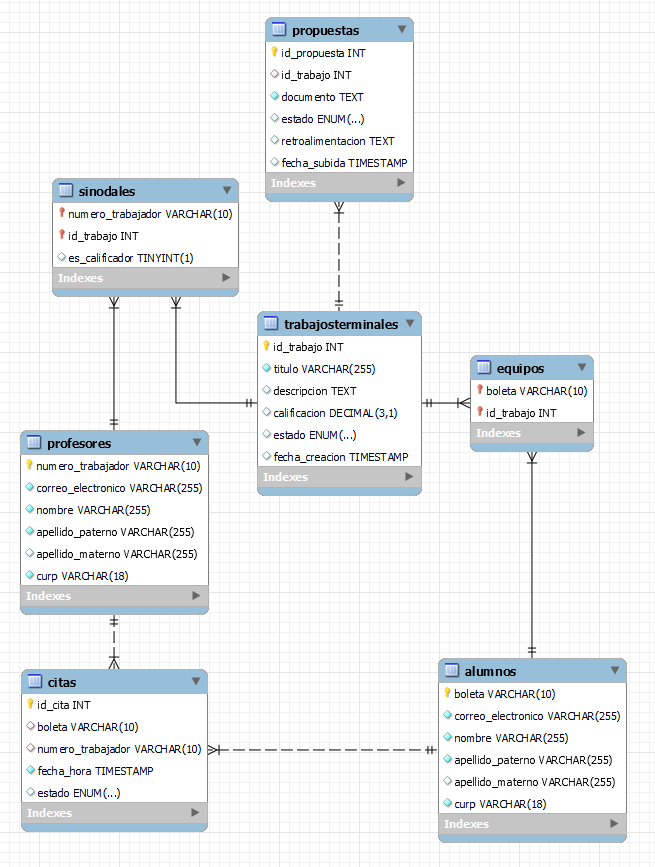
\includegraphics[scale = .87]{bd.png}
\end{figure}
	
\end{document}